\documentclass[a4wide,12pt]{article}

\usepackage{verbatim}
\usepackage{listings}
\usepackage{graphicx}
\usepackage{a4wide}
\usepackage{color}
\usepackage{amsmath}
\usepackage{amssymb}
\usepackage[T1]{fontenc}
\usepackage{cite} % [2,3,4] --> [2--4]
\usepackage{shadow}
\usepackage{hyperref}
\usepackage{fancyhdr}
\usepackage{morefloats}
\pagestyle{fancy}
\rhead{Lars Christian Hauge}


\begin{document}
\section*{Project3}
\subsection*{Abstract}
In this project I have used the Runge-Kutta 4 method to simulate the solar system. I start ith a model of only the Earth and the Sun , before I upgrade it with more planets.
\subsection*{Introduction}
In this project we are supposed to model the solar system. We start easy with just one planet before we add more planets. We have been asked to use the Runge-Kutta 4 method used in the lecture notes and some part of the program should be object-oriented. 

The solar system is relatively easy to simulate as it is only dependent on one force, gravity. Gravity is again only dependent on distance and mass, where the mass is constant. So the differential equations we shall solve will only be dependent on time, position and its derivatives. 

I have included all the plots in the end of the report for better readability, all plots included have a time scale of 100 years, until we come to the escape velocity part where they will have a time scale of a 1000 years.  
\subsection*{Methods}
We started out by defining the equations and writing them as a set of coupled first order differential equations that are possible to solve by the Runge-Kutta 4 method. We have the equations:
\[
\frac{d^{2}x}{dt^{2}} = \frac{F_{G,x}}{M_{Earth}}
\]
and 
\[
\frac{d^{2}y}{dt^{2}} = \frac{F_{G,y}}{M_{Earth}}
\]
from this we get:
\[ 
\frac{dv_{x}}{dt} = \frac{F_{G,x}}{M_{Earth}} , \frac{dv_{y}}{dt} = \frac{F_{G,y}}{M_{Earth}}
\]
and
\[
\frac{dx}{dt} = v_{x} , \frac{dy}{dt} = v_{y}
\]

By first finding the velocity for the different planets in the system and then the position of the planets, we have some equations easily solvable by the Runge-Kutta Method. The Runge-Kutta method goes like this:
\[
y_{i+1} = y_{i} + \frac{1}{6}*(k_{1}+2k_{2}+2k_{3}+k_{4})
\]
where
\[
k_{1} =  hf(t_{i}, y_{i})
\]
\[
k_{2} = hf(t_{i}+\frac{h}{2}, y_{i} + \frac{k_{1}}{2})
\]
\[
k_{3} = hf(t_{i}+\frac{h}{2}, y_{i} + \frac{k_{2}}{2})
\]
\[
k_{4} = hf(t_{i}+h, y_{i}+k_{3})
\]

As a basis for my solution I used the programs already written by Morten Jensen on this website: \url{http://folk.uio.no/mhjensen/compphys/programs/chapter08/cpp/solarsystem/}. 
I made some alterations to the programs and in the end the results became nice. The general idea of the programs are just the same, so I feel no need to list the programs I used in the end. 
The data about the solar system I found at \url{http://nssdc.gsfc.nasa.gov/planetary/factsheet/}. 

\subsection*{Results}
As we see from figure ~\ref{fig:01} and ~\ref{fig:02} the minimum velocity that gives a circular orbit is about $17 \frac{km}{s}$. It gives a slightly strange orbit, but if we increase the velocity we get a more and more circular orbit as you can see in the figures ~\ref{fig:03} and ~\ref{fig:04}. The latter of these two has a speed of $29.29 \frac{km}{s}$ and this is the speed the earth actually have, and we see it is perfectly circular. As this is the speed the earth normally have I will use it for the rest of this exercise. 

I have defined the step length in days, and with a step length of 1 day you get figure ~\ref{fig:04}, if we increase the time step to 5 days we get what we see in figure ~\ref{fig:05}. The plots in figure ~\ref{fig:06} and ~\ref{fig:07} show the orbit for 10 and 20 days as time step. We see that it becomes more and more unruly, and after 20 days it just becomes a straight line. 

We see from figure ~\ref{fig:08} and ~\ref{fig:09} that there are some slight changes in energy and angular momentum. 
These are very small changes compared to their size. In these plots the energy is multiplied by a factor $10^{-30}$ and angular momentum with $10^{-35}$, so the changes we see are
negligible, so we can conclude that energy and angular momentum is conserved. These quantities are conserved because they both are dependent on radius and velocity, and as
\[
v^{2}r = GM_{\odot} = 4\pi^{2}AU^{3}/yr^{2} = constant
\] 
angular momentum and energy must also be constants. 

To see if the Earth escaped from the Sun I increased the initial velocity and plotted the orbit. The orbit did not change significantly before it was $40 \frac{km}{s}$ as seen in figure ~\ref{fig:10}.
I then went carefully upwards and found that at $41.7 \frac{km}{s}$ it behaved really strange (fig. ~\ref{fig:11} and that at $41.8 \frac{km}{s}$(fig. ~\ref{fig:12} the Earth escaped from the sun. 

The figures ~\ref{fig:13}, ~\ref{fig:14} and ~\ref{fig:15} all show the Earth and Jupiter orbiting the Sun for different Jupiter masses. 
As the heaviest Jupiter gave the coolest plots, I chose to use this to test the stability of the Runge-Kutta 4 solver. The solver was really precise,
it was not before the time step hit 20 days I really got something that was not really close to what we have seen in figure ~\ref{fig:15}. Figure ~\ref{fig:16} shows what happened when the time step reached 20.

The last figures from ~\ref{fig:17} to ~\ref{fig:23} are all from the simulation where I ran the entire solar system. The first plot is the entire solar system
and the next plots are of the inner solar system as their orbit are hard to look at in detail. 

We see that the orbits of the planets in the inner solar system and Pluto's are elliptical while the massive planets in the outer solar system have more circular orbits. 
\subsection*{Conclusion}
We have in this exercise seen how we can simulate the solar system by Newton's equations and a simple numerical method like Runge-Kutta 4. 
We saw that the planets made the orbits of the inner planets become more elliptical than when we only modelled the Earth and the Sun. 
The Runge-Kutta 4 method is a really stable numerical method and you can use pretty large time steps and still get nice results. 

\begin{figure}[p]
 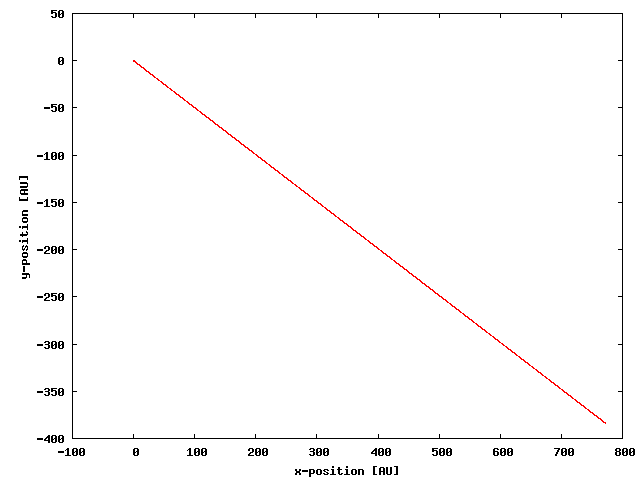
\includegraphics[width=0.5\textwidth]{Earth16km}
 \caption{Orbit of the Earth with an initial velocity of $16 \frac{km}{s}$}
 \label{fig:01} 
\end{figure}
\begin{figure}[p]
 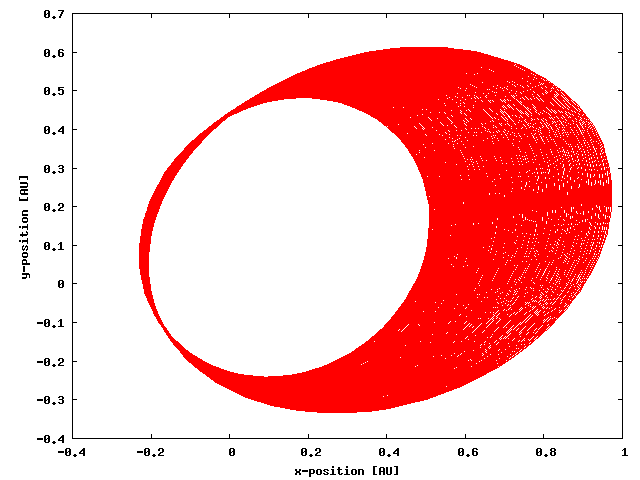
\includegraphics[width=0.5\textwidth]{Earth17km}
 \caption{Orbit of the Earth with an initial velocity of $17 \frac{km}{s}$}
 \label{fig:02} 
\end{figure}
\begin{figure}[p]
 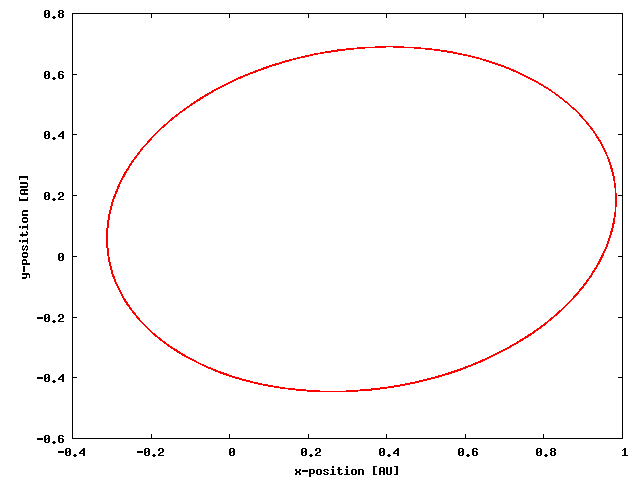
\includegraphics[width=0.5\textwidth]{jord20km}
 \caption{Orbit of the Earth with an initial velocity of $20 \frac{km}{s}$}
 \label{fig:03} 
\end{figure}
\begin{figure}[p]
 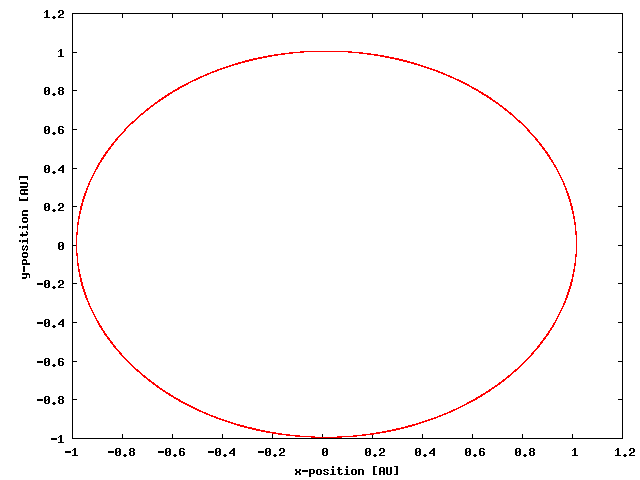
\includegraphics[width=0.5\textwidth]{jordmedsol}
 \caption{Orbit of the Earth with an initial velocity of $29.29 \frac{km}{s}$}
 \label{fig:04} 
\end{figure}
\begin{figure}[p]
 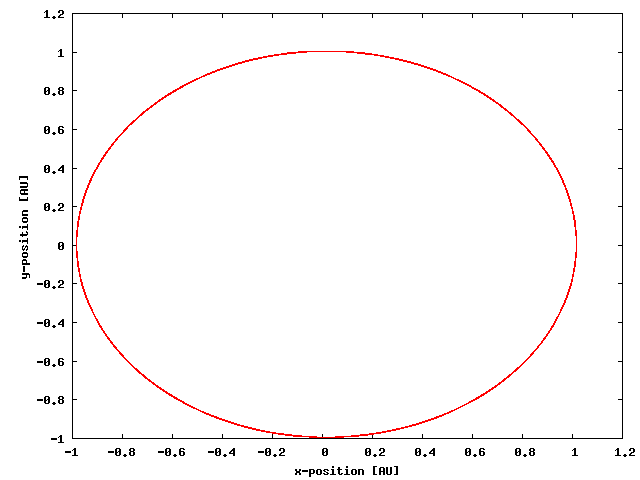
\includegraphics[width=0.5\textwidth]{jordmedsoldt5}
 \caption{Orbit of the Earth with a timestep of 5 days}
 \label{fig:05} 
\end{figure}
\begin{figure}[p]
 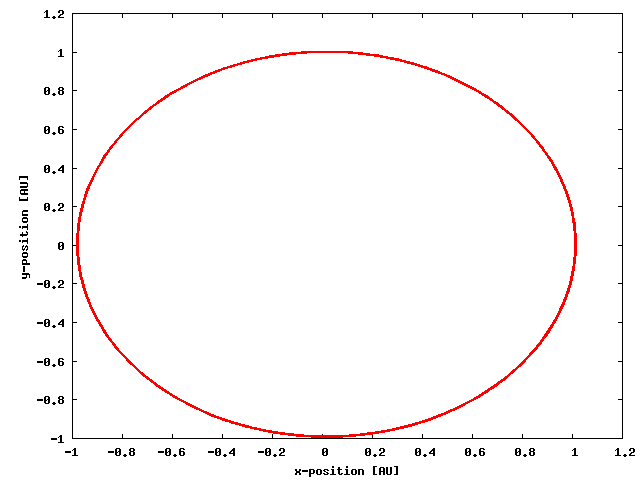
\includegraphics[width=0.5\textwidth]{jordmedsoldt10}
 \caption{Orbit of the Earth with a timestep of 10 days}
 \label{fig:06} 
\end{figure}
\begin{figure}[p]
 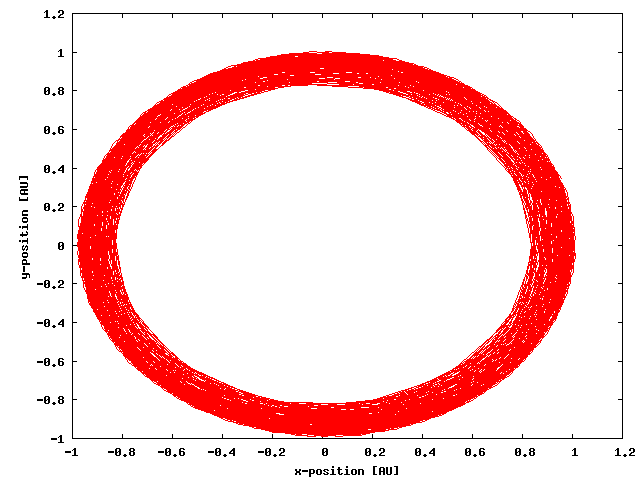
\includegraphics[width=0.5\textwidth]{jordmedsoldt20}
 \caption{Orbit of the Earth with a timestep of 20 days}
 \label{fig:07} 
\end{figure}
\begin{figure}[p]
 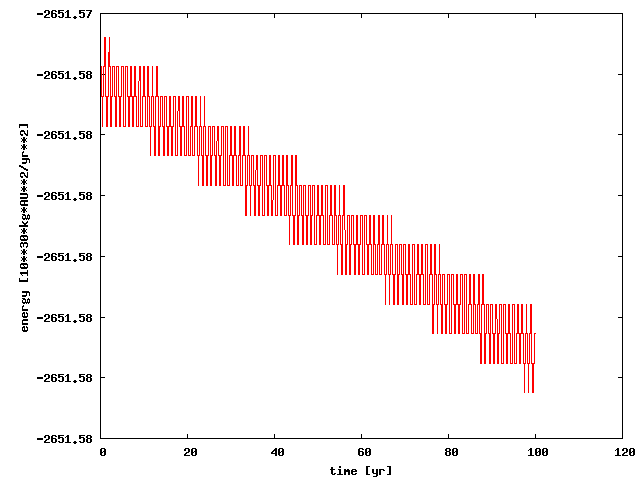
\includegraphics[width=0.5\textwidth]{energy}
 \caption{Earth's energy around the Sun}
 \label{fig:08} 
\end{figure}
\begin{figure}[p]
 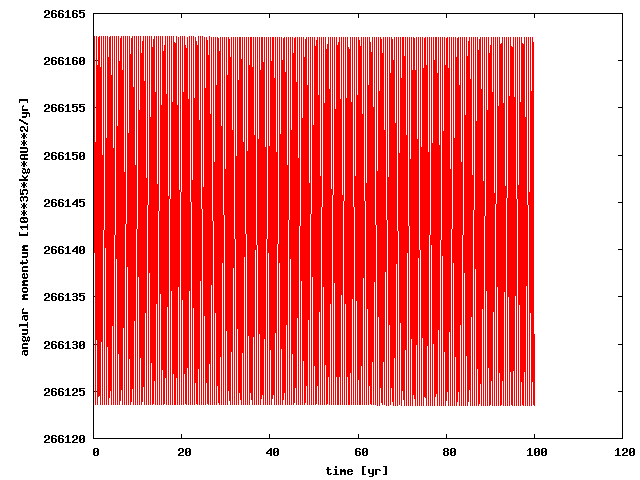
\includegraphics[width=0.5\textwidth]{spin}
 \caption{Earth's angular momentum around the Sun}
 \label{fig:09} 
\end{figure}
\begin{figure}[p]
 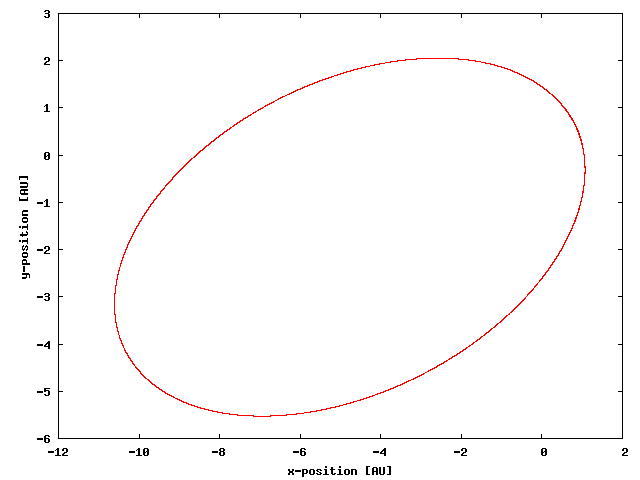
\includegraphics[width=0.5\textwidth]{jordesc40}
 \caption{Orbit of the Earth with initial velocity $40 \frac{km}{s}$}
 \label{fig:10} 
\end{figure}
\begin{figure}[p]
 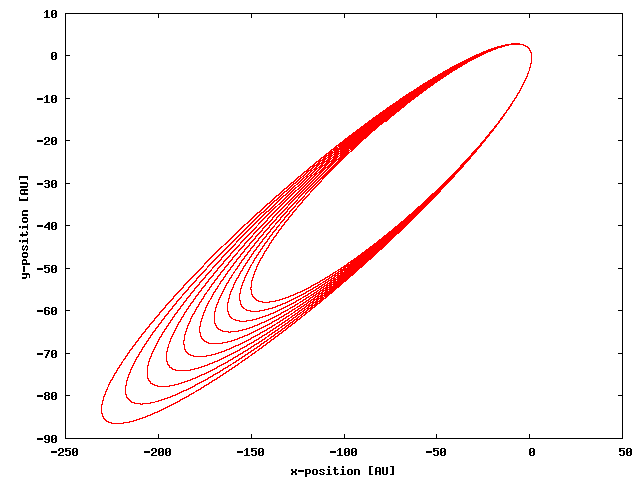
\includegraphics[width=0.5\textwidth]{jordesc417}
 \caption{Orbit of the Earth with initial velocity $41.7 \frac{km}{s}$}
 \label{fig:11} 
\end{figure}
\begin{figure}[p]
 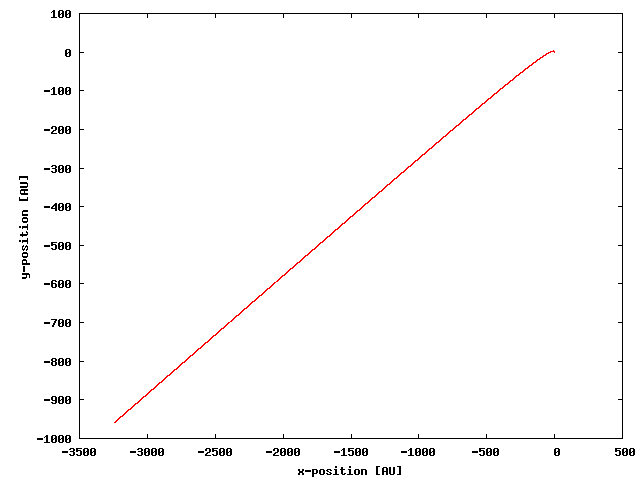
\includegraphics[width=0.5\textwidth]{jordesc42}
 \caption{Orbit of the Earth with initial velocity $41.8 \frac{km}{s}$}
 \label{fig:12} 
\end{figure}
\begin{figure}[p]
 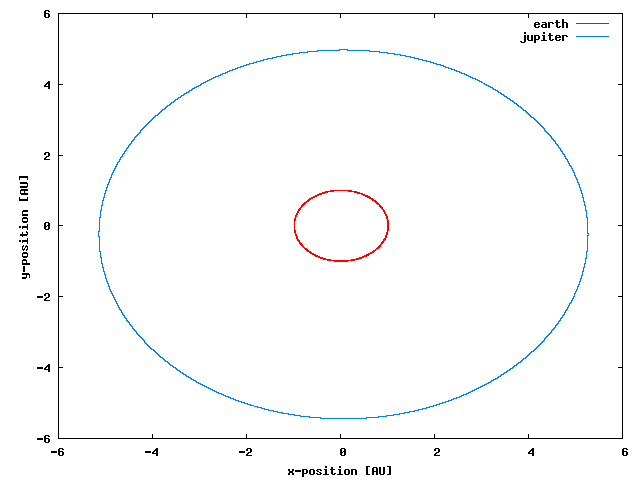
\includegraphics[width=0.5\textwidth]{jordjup}
 \caption{Orbit of Jupiter and Earth around the Sun}
 \label{fig:13} 
\end{figure}
\begin{figure}[p]
 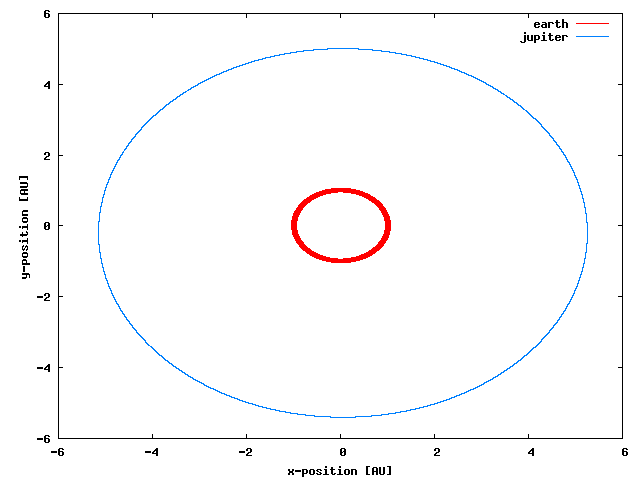
\includegraphics[width=0.5\textwidth]{jordjup10}
 \caption{Orbit of Jupiter and Earth around the Sun, with 10 times more massive Jupiter}
 \label{fig:14} 
\end{figure}
\begin{figure}[p]
 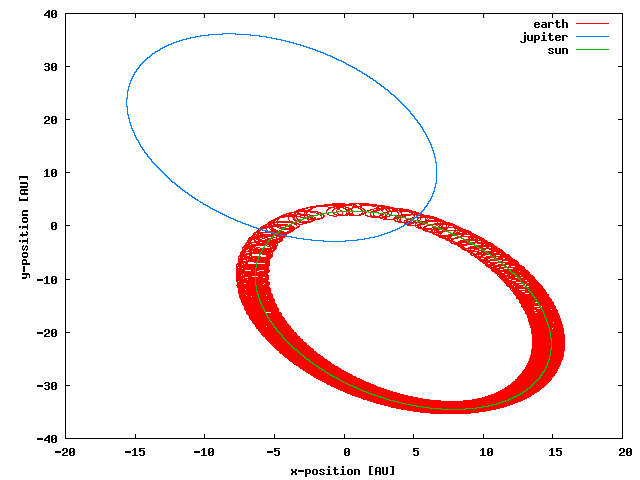
\includegraphics[width=0.5\textwidth]{jordjupsol1000}
 \caption{Orbit of Jupiter, Earth the Sun, with 1000 times more massive Jupiter}
 \label{fig:15} 
\end{figure}
\begin{figure}[p]
 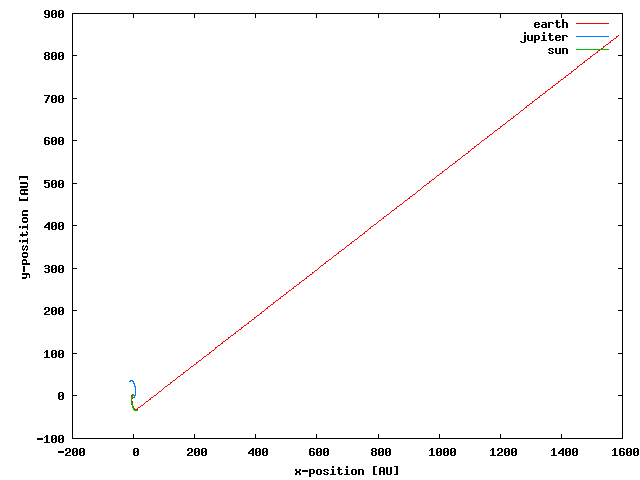
\includegraphics[width=0.5\textwidth]{jordjupsol1000dt202}
 \caption{Orbit of Jupiter, Earth the Sun, with 1000 times more massive Jupiter, time step 20 days}
 \label{fig:16} 
\end{figure}

\begin{figure}[p]
 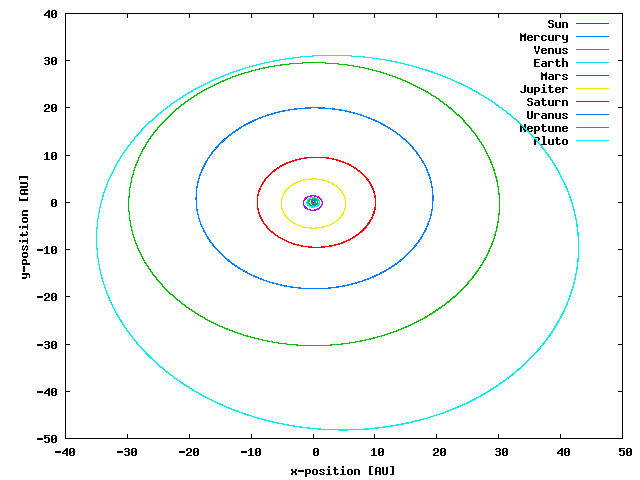
\includegraphics[width=0.5\textwidth]{solarsystem}
 \caption{All the orbits for the planets in the solar system}
 \label{fig:17} 
\end{figure}

\begin{figure}[p]
 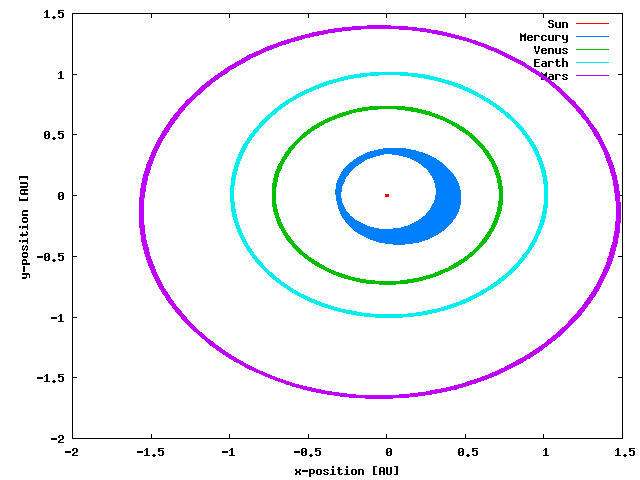
\includegraphics[width=0.5\textwidth]{innersolar}
 \caption{The orbits of the planets in the inner solar system}
 \label{fig:18} 
\end{figure}

\begin{figure}[p]
 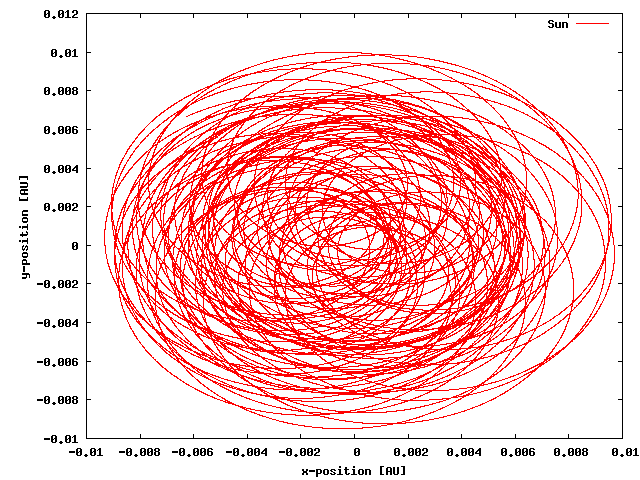
\includegraphics[width=0.5\textwidth]{sun}
 \caption{The motion of the Sun}
 \label{fig:19} 
\end{figure}

\begin{figure}[p]
 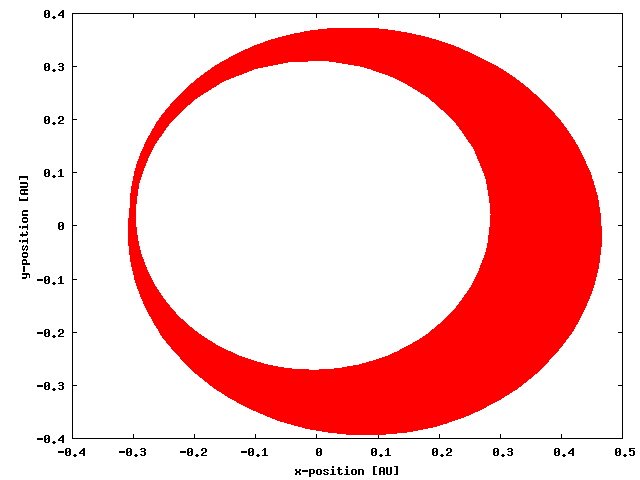
\includegraphics[width=0.5\textwidth]{Mercuryrel}
 \caption{Mercury's orbit}
 \label{fig:20} 
\end{figure}

\begin{figure}[p]
 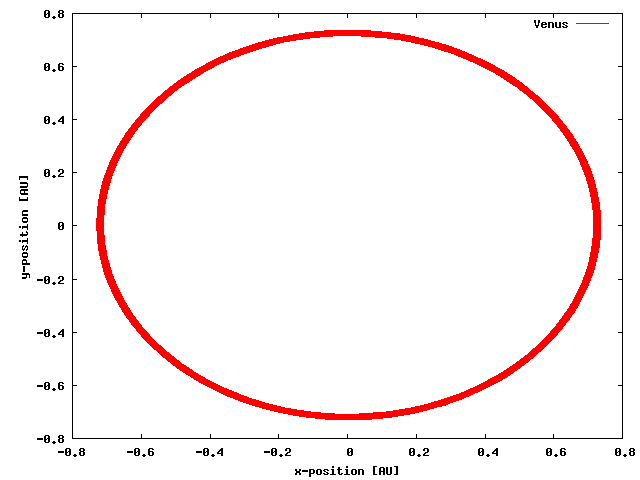
\includegraphics[width=0.5\textwidth]{venus}
 \caption{Venus' orbit}
 \label{fig:21} 
\end{figure}

\begin{figure}[p]
 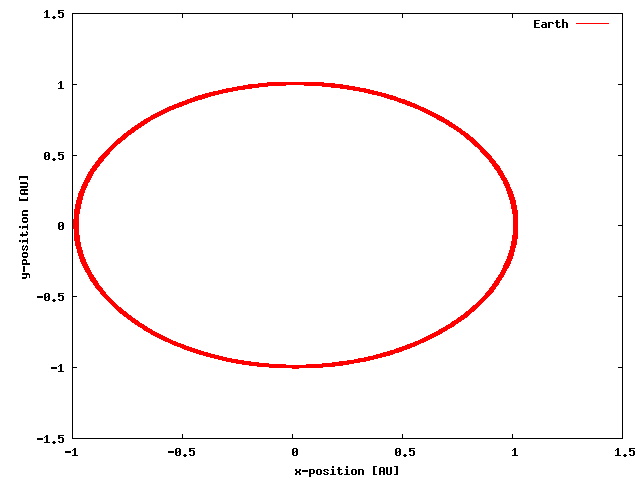
\includegraphics[width=0.5\textwidth]{Earth}
 \caption{Earth's orbit}
 \label{fig:22} 
\end{figure}

\begin{figure}[p]
 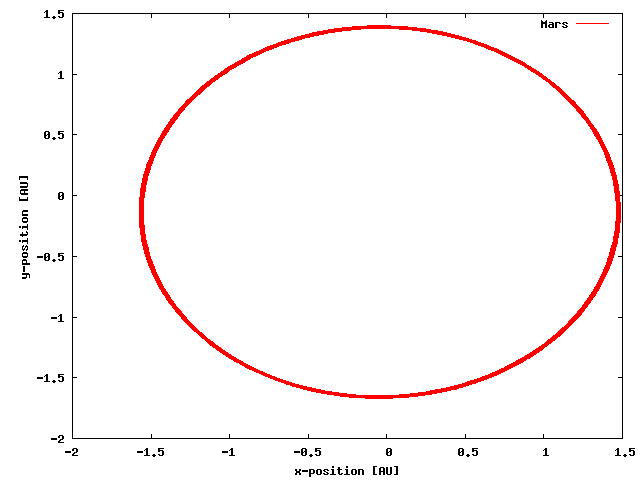
\includegraphics[width=0.5\textwidth]{Mars}
 \caption{Mars' orbit}
 \label{fig:23} 
\end{figure}

\end{document}




